STMs may be operated at very different temperatures. The lowest temperature is only limited by the availability of sufficient cooling. While low temperature (LT) STMs may be operated with solely helium, it is more resource-saving to cool the direct proximity of the sample and the STM with He, but to suppress the heat flow out of the He-cryostat with a second surrounding nitrogen cryostat (boiling point: \SI{77}{\K}, compare figure \ref{fig:STM-cryo}). This diminishes consumption of globally limited and rather expensive He. To maintain a temperature of \SIrange{5}{7}{\K}, one to two liters of liquid helium are required a day, plus an additional amount of three to four liters liquid nitrogen. Evaporated helium is reclaimed in a closed circuit with a system of purifying and storage/cooling steps so that only a small amount of helium escapes the circuit and is lost.

Sample temperatures down to \SIrange{5}{7}{\K} allow for observations not possible at elevated (room) temperature. While cooling not only reduces thermal drift in the piezo elements that are used to determine the tip's position on the sample. Thermal energy at low temperature is not high enough for atoms or molecules to move on the surface. Species mobile at room temperature (and therefor not representable at room temperature) are now immobile and accessible for STM imaging and spectroscopy.

\begin{figure}[ht]
	\begin{center}
		\subfigure[LT-STM setup]{
			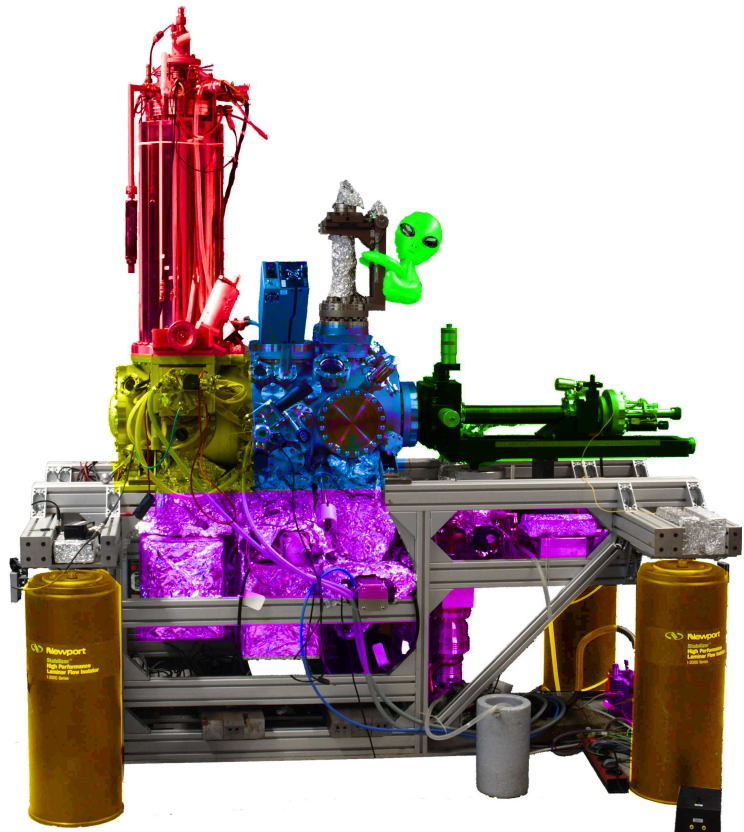
\includegraphics[width=0.45\textwidth]{./images/chamber-sketch.jpg}
			\label{fig:STM-modes}
		}
		\subfigure[Sheme of STM liquid bath cryostats]{
			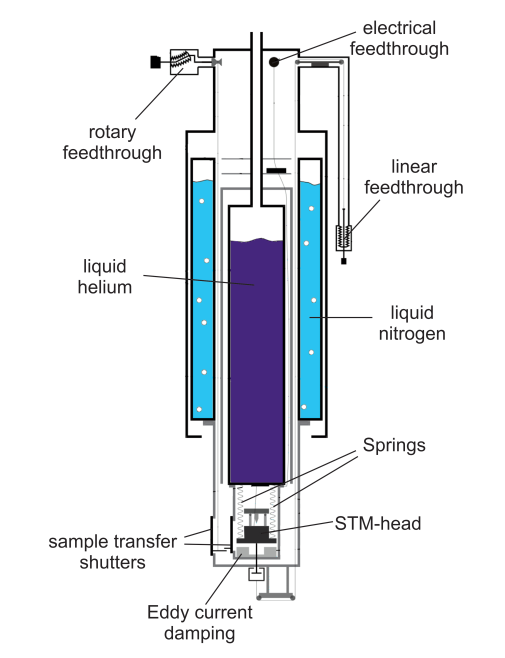
\includegraphics[width=0.45\textwidth]{./images/sketch-cryo.jpg}
			\label{fig:STM-cryo}
		}
	\end{center}
	\caption{Taken from \cite{diss-manuela} and \cite{diss-knud}}
	\label{fig:STM}
\end{figure}